Understanding how atoms or molecules respond to irradiation with x-rays gives insight into the structure of solutions (Ref.\ \citep{smith17:13909} and references therein), and the mechanisms of radiation damage \citep{ONeill02:329,Carugo05:213,Stumpf16:237}. Depending on the photon energy, the absorption of an x-ray photon results in the population of core-excited or core-ionized states. The relaxation of these highly energetic states involves an ultrafast cascade of intraatomic processes, such as radiative and Auger decays, and it depends on the character of the initially populated states \citep{stoychev08:074307,Demekhin08:043421,Demekhin09:104303,Ouchi11:053415,Miteva14:164303,travnikova16:213001,Gokhberg14:661,Trinter14:664}. Furthermore, if the initially excited or ionized species is embedded in an environment, interatomic processes are possible  \citep{Pokapanich09:7264,Pokapanich11:13430,Stumpf16:237,unger17:708,ceolin17:263003}.


%X-ray absorption spectroscopy (XAS) is a powerful tool to study the nearest environment of atoms in gas phase as it probes core-excited states below threshold which are highly sensitive to the surrounding. However, for atoms and molecules in liquid or solid phase, these core-excited states overlap significantly in the XAS spectra inhibiting access to the available information {\color{red}(REF)}. This drawback can be overcome by detecting the electrons resulting from the subsequent resonant Auger decay and thus using this complementary information to separate the overlapping states \citep{goldsz16:15133}. In a liquid jet, this method applied to shallow core holes (like O 1s of the water molecule) mainly provides information from sites close to the liquid-solid interface, due to the short mean free path of the low-kinetic-energy Auger electrons. With a recently commissioned setup using tender X-rays \citep{ceolin13:188,rueff15:175} we are now able to reach deeper core levels resulting in much faster Auger electrons, and as a consequence, one can have a significantly deeper look into the liquid. 

%X-ray absorption spectroscopy (XAS) applied to gas phase is a powerful tool to describe (de)localized core-excited states associated to a specific atom. In condensed phase studies, these core-excited states overlap significantly inhibiting a simple description of the nearest environment of the targeted atom. This drawback can be overcome by detecting the electrons resulting from the subsequent resonant Auger decay and by using this complementary information to separate the overlapping states \citep{goldsz16:15133}. 
{\color{red}X-ray absorption spectroscopy (XAS) in the soft x-ray regime is a powerful tool to describe core-excited states of a specific atom and thus to probe its electronic structure and the local environment surrounding it. In the tender and hard x-ray regimes, due to the lifetime broadening, these core-excited states overlap significantly inhibiting a simple description of the nearest environment of the targeted atom. This drawback can be overcome by detecting the electrons resulting from the subsequent resonant Auger decay and by using this complementary information to separate the overlapping states \citep{foehlisch05:373,goldsz16:15133}.}
With our recently commissioned microjet setup dedicated to the study of liquids by means of the photoemission technique using tender x-rays \citep{ceolin13:188,rueff15:175}, we are now able to probe much deeper core levels and corresponding fast Auger electrons. This allows us to focus our investigations on the liquid bulk by strongly reducing the specific interface contributions, and also to access ultrafast dynamical processes owing to the very short lifetimes of the corresponding core-excited states.


In this work we combine Auger electron spectroscopy (AES) together with XAS in the tender x-ray regime to study the electronic decay processes following x-ray absorption of aqueous potassium chloride at the K-edges of both \ki~and \cli. In particular, we demonstrate experimentally that at photon energies below the K-edges of the two ions, core-excited states are populated. These states undergo resonant Auger decay within less than 1\,fs \citep{ceolin17:263003}. Although the \ki~and \cli~ions are isoelectronic, they have different fingerprints in the resonant Auger spectra. We demonstrate that these differences result from different electronic structures of the two ions, thus confirming that the combination of XAS and AES techniques is a sensitive probe of the electronic structure of solutions.


\begin{figure}
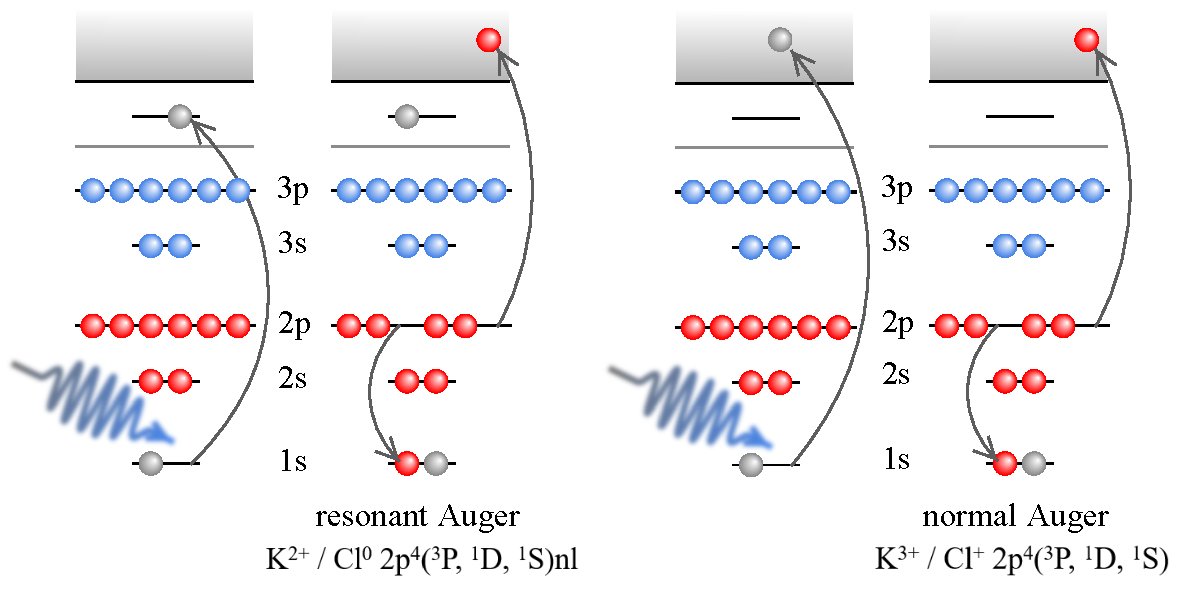
\includegraphics[scale=0.8]{figures/auger_process.pdf}
\caption{Schematic representation of the resonant (left) and normal (right) Auger processes of the isoelectronic \ki~and \cli~ions.}
\label{fg:auger}
\end{figure}

The resonant and normal Auger spectra of K$^+_{\rm aq}$ and Cl$^-_{\rm aq}$ were measured using a newly operational microjet setup designed for the HAXPES end station of the GALAXIES beamline at the synchrotron radiation facility SOLEIL in France \citep{ceolin13:188,rueff15:175}; for details, see Supplementary Information (SI). 
{\color{red}The spectra are presented on Figs.\ \ref{fg:2dmap_k} and \ref{fg:2dmap_cl} as 2D maps, showing the dependence of the kinetic energy of the Auger electron on the incoming photon energy.}
The investigated Auger processes are schematically shown on Fig.\ \ref{fg:auger}. The KL$_{2,3}$L$_{2,3}$ normal Auger decay of aqueous \ki~and \cli~populates the 2p$^{-2}$($^3$P, $^1$D, $^1$S) final states. The transitions to $^3$P final states are weak since they are forbidden in LS coupling. For K$^{+}_{\text{aq}}$ the maxima of the $^1$S and $^1$D Auger lines for a photon energy h$\nu = 3616.0$\,eV are located at kinetic energies $E_{\text{kin}} = 2958.0$\,eV and 2968.5\,eV, respectively (Fig.\ \ref{fg:2dmap_k}(c)). For Cl$^{-}_{\text{aq}}$, the lines corresponding to the Cl$^{+}$ 2p$^{-2}$($^1$S) and ($^1$D) states are located at $E_{\text{kin}} = 2373.1$\,eV and 2382.0\,eV for h$\nu = 2830.0$\,eV (Fig.\ \ref{fg:2dmap_cl}(c)). Close to threshold the KL$_{2,3}$L$_{2,3}$ normal Auger lines are asymmetric and also shifted to higher kinetic energies as compared to the spectra reported in \citep{ceolin17:263003}. This is due to post-collision interaction \citep{russek86:911,guillemin15:012503}, which is discussed in more detail in the SI.


\begin{figure}[h!]
\centering
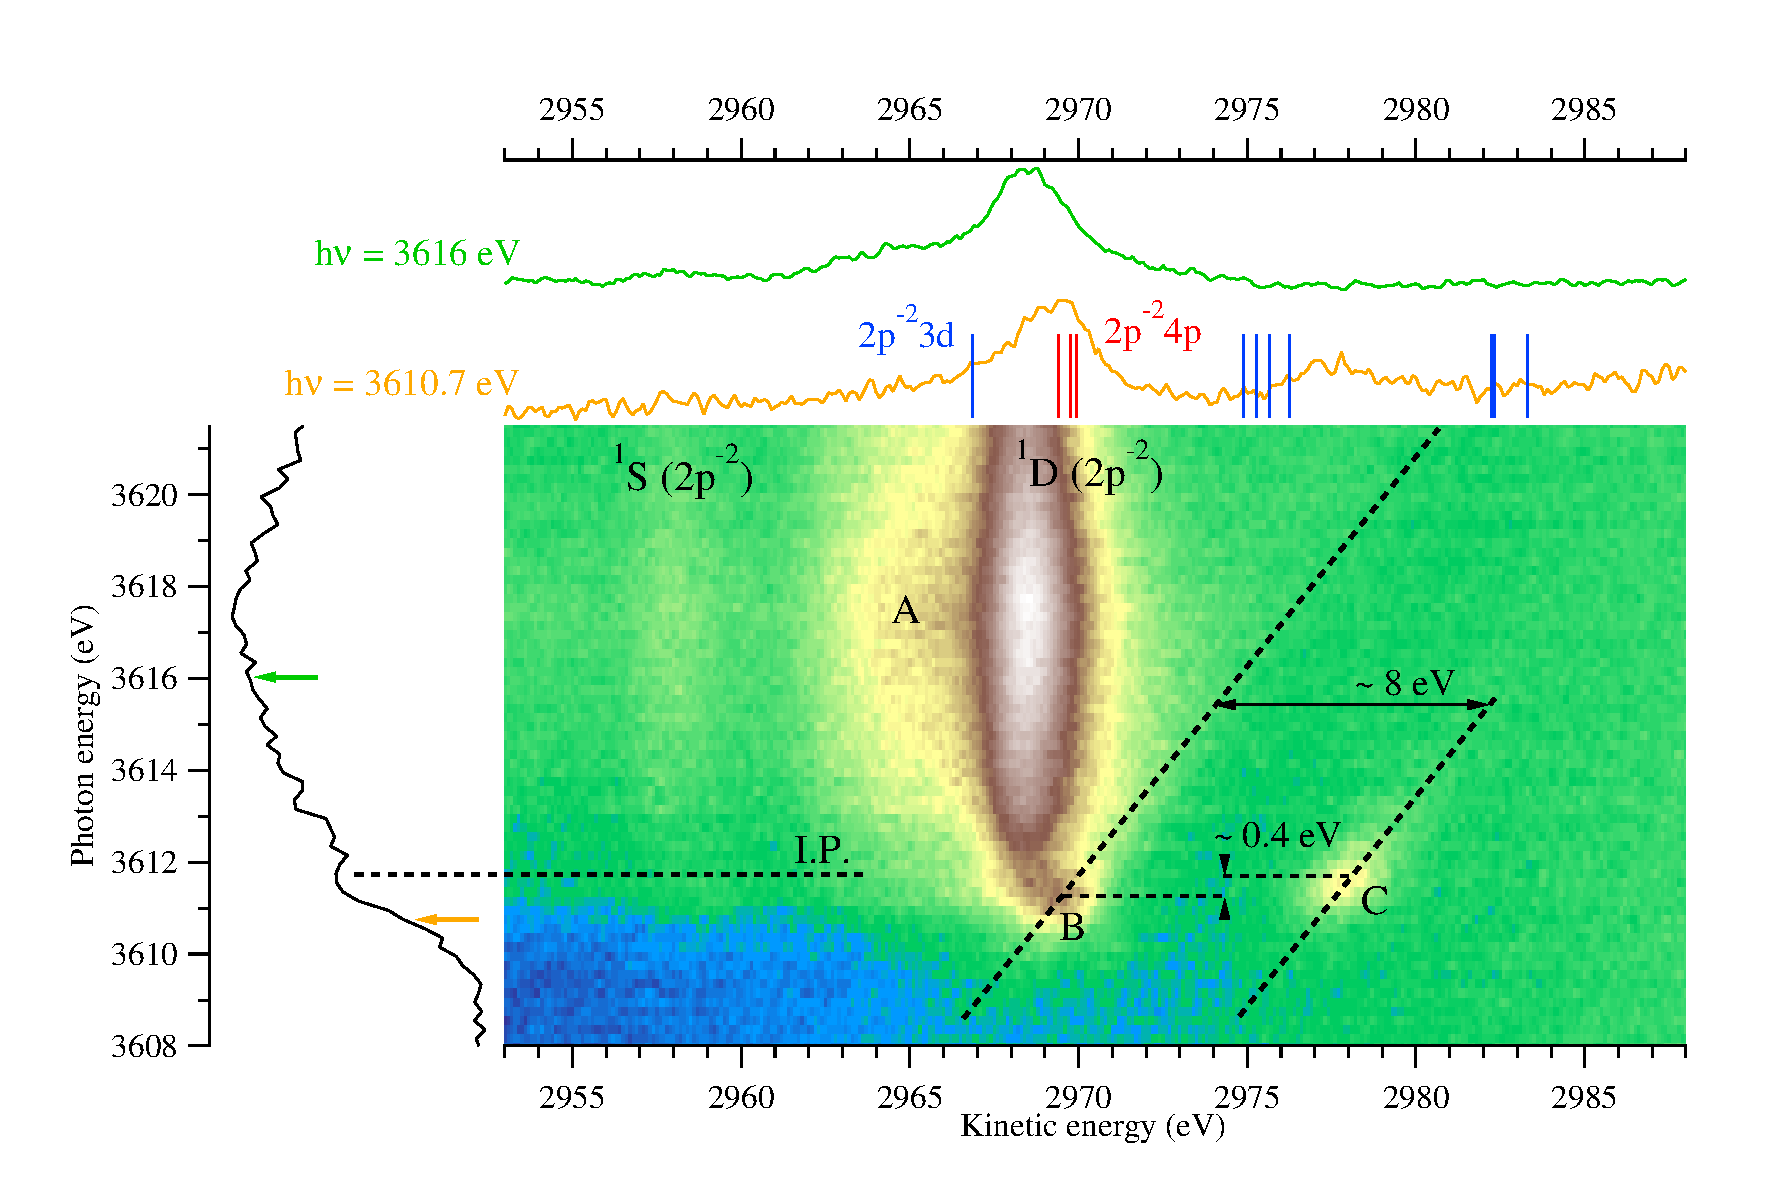
\includegraphics[scale=0.55]{figures/k_2dmap.pdf}
\caption{(a) 2D map showing the kinetic energy of the electrons emitted in KL$_{2,3}$L$_{2,3}$ Auger decay vs the photon energy in the vicinity of the K-edge of aqueous K$^{+}$. The features A, B and C are discussed in the text.
(b) Experimental partial electron yield spectrum of K$^{+}$ obtained after integrating over the kinetic energies of the Auger electrons.
(c) Auger spectra at photon energies 3610.7\,eV and 3616\,eV. The vertical bars in the resonant Auger spectrum measured at 3610.7\,eV indicate the spectator Auger energies of the calculated doublet 2p$^{-2}$ 3d (blue) and 2p$^{-2}$4p (red) states of K$^{+}$(H$_2$O)$_6$.}
\label{fg:2dmap_k}
\end{figure}


Finally, the normal Auger $^1$D main line of K$^{+}$ differs from that of Cl$^{-}$ by the presence of a large shoulder on the low kinetic-energy side at $E_{\text{kin}} \cong 2965$\,eV, feature A (Fig.\ \ref{fg:2dmap_k}(a)). This shoulder is attributed to electron transfer from the solvent water molecules to the unoccupied 3d orbitals of K$^{3+}$(2p$^{-2}$) resulting in K$^{2+}$(2p$^{-2}$3d)W$^{+}$ \citep{ceolin17:263003}. In the case of \cli, there is no experimental evidence of such intense electron transfer processes.


\begin{figure}[h!]
\centering
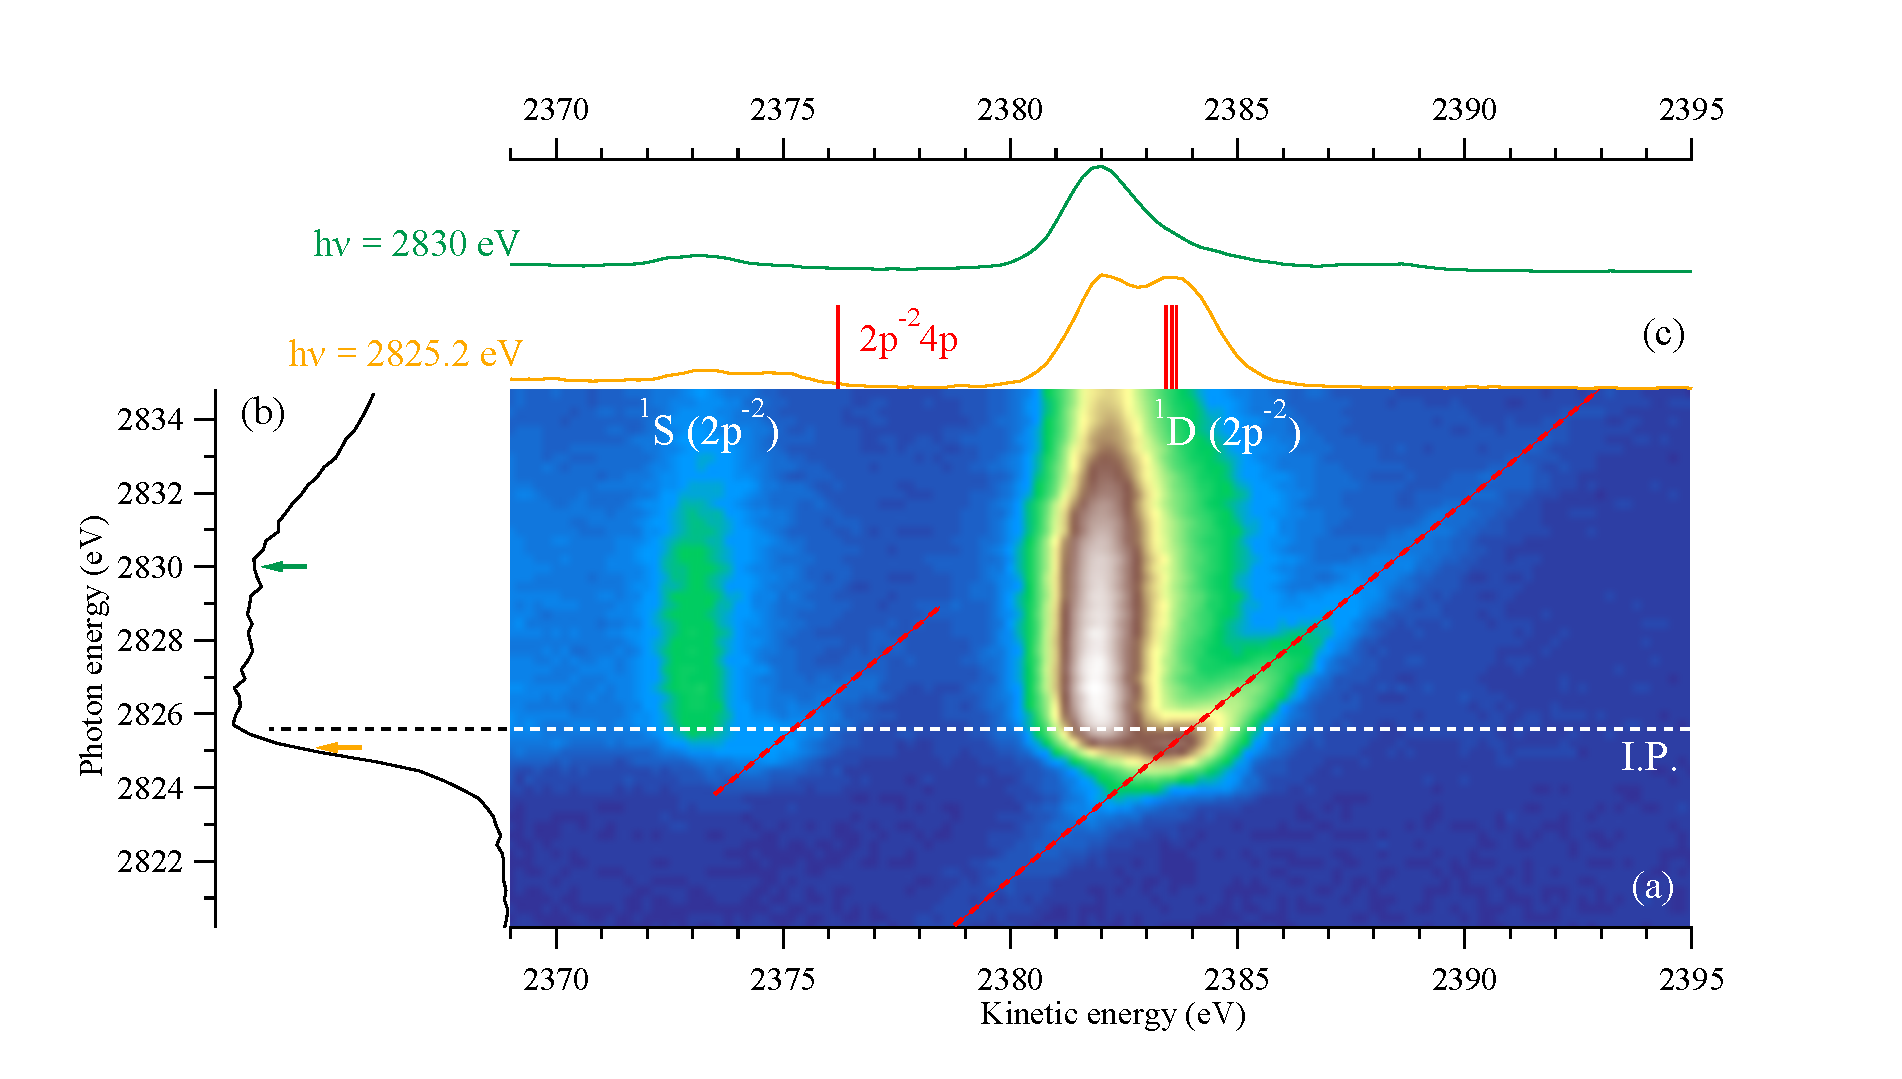
\includegraphics[scale=0.55]{figures/cl_2dmap.pdf}
\caption{(a) 2D map showing the kinetic energy of the electrons emitted in KL$_{2,3}$L$_{2,3}$ Auger decay vs the photon energy in the vicinity of the K-edge of aqueous Cl$^{-}$. 
(b) Experimental partial electron yield spectrum of Cl$^{-}$ obtained after integrating over the kinetic energies of the Auger electrons. 
(c) Auger spectra at photon energies 2825.2\,eV and 2830.0\,eV. The vertical bars in the resonant Auger spectrum at 2825.2\,eV indicate the the spectator Auger energies of the calculated doublet 2p$^{-2}$4p states of Cl$^{-}$(H$_2$O)$_6$.}
\label{fg:2dmap_cl}
\end{figure}


The pre-edge regions of the XAS spectra of \ki~and \cli~shown in Figs.\ \ref{fg:2dmap_k}(b) and \ref{fg:2dmap_cl}(b) do not show any clear indication of core-excited states due to their lifetime broadening and energetic proximity to the ionization threshold. However, these states can be identified by their resonant Auger features, which disperse with photon energy and thus significantly differ from the normal Auger ones. In the 2D map of \cli~(Fig.\ \ref{fg:2dmap_cl}(a)) there are two dispersive resonant Auger features indicated with diagonal dashed lines. Both of them have a maximum at $h\nu =  2825.2$\,eV, which is in good agreement with the position of the Cl$^{-}$ 1s$^{-1}$4p excitation determined from Cl K-edge XAS experiments on hydrated Mg and Sr chlorides\citep{sugiura82:681} and metal-chloride complexes \citep{shadle95:2259}. The dispersive features have $E_{\text{kin}} = 2374.6$ and 2383.4\,eV relating them to the $^1$S and $^1$D main lines, respectively. In the case of \ki, the dispersive line related to the $^1$S main line cannot be clearly identified due to the presence of a strong background. Instead two dispersive features related to the $^1$D main line are observed denoted as B and C on Fig.\ \ref{fg:2dmap_k}(a). Feature B exhibits a maximum at h$\nu = 3611.2$\,eV and $E_{\text{kin}} = 2969.2$\,eV. The additional feature C appears at h$\nu = 3611.6$\,eV and $E_{\text{kin}} = 2978.1$\,eV, thus it is separated by approximately 400\,meV in photon energy and 8.3\,eV in kinetic energy from the maximum of feature B. The positions of these two core-excited states are close to the energy of the 1s$^{-1}$4p excitation of gas-phase \ki~-- 3610.7\,eV \citep{hertlein06:062715}.


\begin{figure}[h!]
\centering
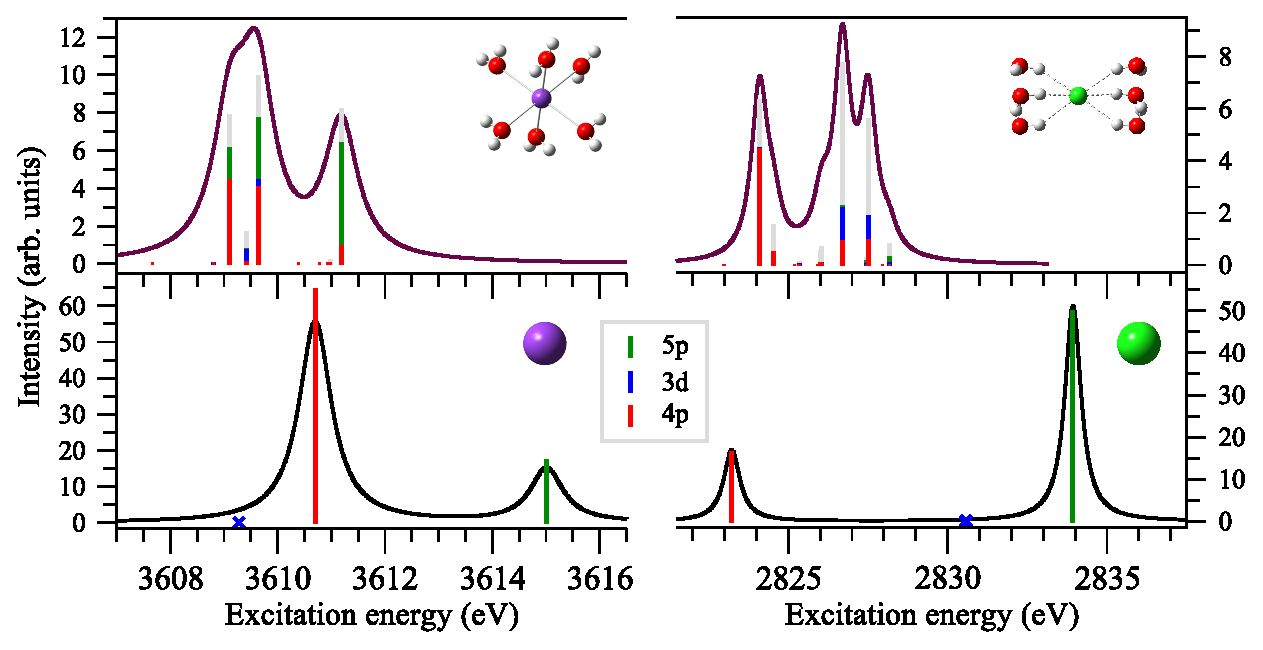
\includegraphics[scale=0.55]{figures/xas_spectra.eps}
\caption{XAS spectra of the lowest K-shell resonant transitions in the isolated K$^{+}$ (a) and Cl$^{-}$ (b) ions and their 6-coordinated clusters, (c) and (d). For comparison with the experiment, the theoretical stick spectra are convolved with a Lorentzian of FWHM 0.74\,eV and 0.62\,eV representing the lifetime broadening of \ki~and \cli \citep{Krause79:329} (dashed lines) and a Voigt profile (solid line) to account for both the lifetime and the experimental broadening (see text). The colors in the stick spectrum represent the projections of the singly-occupied natural orbitals (SONOs) of the core-excited 6-coordinated clusters on the basis of SONOs belonging to the 1s$^{-1}$3d, 1s$^{-1}$4p, and 1s$^{-1}$5p states of the isolated ions. The remaining contributions from higher-lying atomic core excitations or from excitations to the solvent molecules are depicted as grey sticks. The theoretical XAS spectra of both \ki~and \cli~were shifted to higher photon energies such that the energies of the lowest core-excited states correspond to the experimentally determined ones. The experimental ionization thresholds are depicted as grey boxes.}
\label{fg:xas_kcl}
\end{figure}


In order to rationalize the pre-edge region of the experimental XAS spectra and the differences in the AES spectra of \ki$_{\text{aq}}$ and \cli$_{\text{aq}}$, we computed the lowest core-excited states of the isolated \ki~and \cli~ions and their hexa-coordinated clusters using the algebraic diagrammatic construction method for the polarization propagator \citep{sch82:2395} within the core-valence separation approximation \citep{bar85:867,ced80:206,ced81:1038} (CVS-ADC(2)x) as implemented in the Q-Chem package \citep{Wenzel14:1900,Wenzel14:4583,Wormit14:774,QChem2015} (see SI for details). The theoretical XAS spectra of the isolated ions (Fig.\ \ref{fg:xas_kcl}(a),(b)) show the two dipole-allowed states, 1s$^{-1}$4p and 1s$^{-1}$5p, which are split by 4.3\,eV and 10.8\,eV in \ki~and \cli, respectively. For both ions, the energy positions of the dipole-forbidden 1s$^{-1}$3d states are marked with blue crosses. It is noteworthy that the positions of the 1s$^{-1}$4p and 1s$^{-1}$3d states are inverted in \ki~and \cli, and moreover, the splitting between these states is about two times smaller in \ki. These findings are crucial for understanding the Auger spectra of the two ions as shown below. Upon addition of water molecules, the degeneracy of the states is lifted and they interact with other states of the ion or the neighboring water molecules (Fig.\ \ref{fg:xas_kcl}(c),(d)). Thus, dipole-forbidden states acquire intensity in the cluster. A similar effect was observed in the XAS spectra of microsolvated clusters of Na$^{+}$ and Mg$^{2+}$ \citep{miteva16:16671}. %Details on the calculations of the XAS spectra are given in the SI.


Further by comparing the experimental and theoretical XAS spectra, we assume that only the states of the lowest peak in the theoretical XAS spectra are populated in the experiment. In the 6-coordinated \ki~cluster the lowest peak in the spectrum contains three states (Fig.\ \ref{fg:xas_kcl}(c)). The lowest- and highest-lying states are split by approximately 0.5\,eV and they have mixed 4p and 5p character while the low-intensity state in between has a predominantly 1s$^{-1}$3d character. Since the dispersive feature B appears at low excitation energies, we assume that it is produced in the resonant Auger decay of the lowest core-excited states of \ki~of predominantly 1s$^{-1}$4p character. Moreover, we can attribute the feature C to the resonant Auger decay of the low-intensity dipole-forbidden 1s$^{-1}$3d state. Thus, we explain both the energy splitting of $\sim$400\,meV photon energy of B and C, and the fact that island C has lower intensity than B (Fig.\ \ref{fg:2dmap_k}). In the hexa-coordinated cluster of \cli, the solvent molecules have little influence on the position and character of the first state -- it has mainly \cli~1s$^{-1}$4p character with some admixture of states of the nearest water molecules (Fig.\ \ref{fg:xas_kcl}(d)). Consequently, we attribute the two dispersive features associated with the $^1$S and $^1$D main lines on the 2D map of \cli~to the resonant Auger decay of this core-excited state. %involving mostly the 4p orbitals of chloride.


To fully characterize the dispersive features on the experimental 2D maps, we also computed the lowest doublet states of the type K$^{2+}$[2p$^{-2}$nl](H$_2$O)$_6$ and Cl$^{0}$[2p$^{-2}$nl](H$_2$O)$_6$ at the Configuration Interaction Singles (CIS) level using the GAMESS-US package \citep{GUGA_PhysScr_21,GUGA_JCP_70,GUS} (see SI for details). These states are the final states of the spectator Auger decay, which is the predominant decay process for the low-lying core-excited states in isoelectronic argon \citep{ceolin15:022502}. The energy positions of the states (see bars on Figs.\ \ref{fg:2dmap_k}(c) and \ref{fg:2dmap_cl}(c)) are adjusted to the kinetic-energy scale of the Auger spectra of both ions such that the lowest 2p$^{-2}$($^1$D)4p states coincide with the maxima of the dipsersive features related to the $^1$D main line. For \ki(H$_2$O)$_6$ the calculated 2p$^{-2}$4p states are lower in energy by $\sim$5 and 12-13\,eV than two groups of 2p$^{-2}$3d states. Thus, the transitions to the group of 2p$^{-2}$3d final states at $E_{\text{kin}}\cong 2975$\,eV are closer to the kinetic energy of island C. Consequently, we attribute this dispersive feature as originating from the resonant Auger decay of the 1s$^{-1}$3d excitation to this group of 2p$^{-2}$3d states. The theoretical splitting between the 2p$^{-2}$4p and 2p$^{-2}$3d states is smaller than that between islands B and C. This disagreement can be explained with the fact that we consider a single geometry with a fixed number of water molecules in the first solvation shell. Moreover, we do not theoretically account for the effect of distant solvent shells. We assume that the transitions to the 2p$^{-2}$3d states with kinetic energies between 2982 and 2983\,eV have negligible Auger rates since no additional experimental features are observed.


Another argument supporting the assignment of feature C to the 1s$^{-1}$3d $\rightarrow$ 2p$^{-2}$3d Auger transition is the energy difference between the spectral features A and C. Feature A originates from electron transfer processes from water molecules (W) to the doubly core-ionized potassium ion and has the configuration K$^{2+}$(2p$^{-2}$3d)W$^{+}$. The lowest ionization potential of liquid water is about 11.16\,eV \cite{winter04:2625} which matches well the observed A-C splitting. Thus, the above energetic arguments corroborate the attribution of island C as originating from resonant Auger decay to the K$^{2+}$ 2p$^{-2}$3d final states.


In the computed Cl$^{0}$[2p$^{-2}$nl](H$_2$O)$_6$ spectrum there are two groups of states split by about 7\,eV (Fig.\ \ref{fg:2dmap_cl}(c)) corresponding to the 2p$^{-2}$($^1$S)4p and 2p$^{-2}$($^1$D)4p final states. The calculated splitting is in good agreement with the one between the dispersive features on the high kinetic-energy sides of the $^1$S and $^1$D main peaks on Fig.\ \ref{fg:2dmap_cl}(a). Consequently, we assign these features to the 1s$^{-1}$4p $\rightarrow$ 2p$^{-2}$($^1$S, $^1$D)4p resonant Auger transitions of Cl$^{-}_{\text{aq}}$.


The delocalization of core-excited electrons in aqueous solutions is ultrafast and as such it competes with the resonant Auger decay \citep{Nordlund07:217406,ottosson12:1}. To estimate the delocalization time of the core-excited electron, $\tau_{\text{CT}}$, at the pre-edges of K$^{+}$~and Cl$^{-}$, we used the core-hole clock method \cite{bjorneholm92:1892,karis96:1380,wurth00:141,bruehwiler02:703,foehlisch05:373}. Our analysis, presented in detail in SI, shows that in the case of \cli, $\tau_{\text{CT}}$ is of the same order as the Auger lifetime, i.e.\ $\sim$1\,fs. The treatment is more complex in the \ki~case due to the presence of multiple competing processes. However, one can expect much less efficient delocalization in \ki~because the core-excited states appear 1.2\,eV below the ionization threshold compared to 0.2\,eV for chloride and, moreover, the lifetime of the K1s core hole is shorter than for chloride (0.9 vs.\ 1\,fs).


In summary, we studied the electronic structure of aqueous solution of KCl at the K-edges of both K$^{+}_{\text{aq}}$ and Cl$^{-}_{\text{aq}}$ by combining XAS and AES in the tender x-ray regime, and {\it ab initio} calculations. The Auger electron spectra of both ions exhibit features of normal and resonant Auger processes. The spectator resonant Auger decay following the 1s$^{-1}$4p excitation proceeds similarly for both aqueous K$^{+}$ and Cl$^{-}$ resulting in dispersive lines with maxima close to the normal Auger features. However, there is a clear difference between the two ions due to the non-negligible excitation of the dipole-forbidden 1s$^{-1}$3d state of \ki~in solution. The spectator Auger decay of this state produces an additional feature which is well separated from the remaining Auger features. These results are an important first step in the study of relaxation cascades triggered by x-ray photoabsorption in liquids. The Auger processes considered here are inevitably followed by multiple intra- and interatomic electronic decays, such as interatomic Coulombic decay (ICD) and electron-transfer mediated decay (ETMD) \citep{unger17:708,Stumpf16:237}. As a result of the latter processes, genotoxic free radicals and slow electrons are formed in the vicinity of the metal center. The magnitude of the damage inflicted upon the environment and the energies of the emitted electrons depend on the initial Auger step, and can therefore be controlled by tuning the energy of the radiation. Consequently, the results of this work can have implications in understanding radiation chemistry and radiation damage in biologically relevant systems in which metallic centers are ubiquitous.